\documentclass[conference]{IEEEtran}
\IEEEoverridecommandlockouts

\usepackage{cite}
\usepackage{amsmath,amssymb,amsfonts}
\usepackage{algorithmic}
\usepackage{graphicx}
\usepackage{textcomp}
\usepackage{xcolor}
\usepackage{listings}
\usepackage{pgfplots}
\usepackage{booktabs}

\pgfplotsset{compat=1.18}

% Python Code Formatting
\lstset{
    language=Python,
    basicstyle=\ttfamily\footnotesize,
    keywordstyle=\color{blue}\bfseries,
    stringstyle=\color{red},
    commentstyle=\color{green!50!black}\itshape,
    showstringspaces=false,
    breaklines=true,
    frame=single,
    backgroundcolor=\color{gray!5},
    numbers=left,
    numberstyle=\tiny\color{gray},
    xleftmargin=15pt
}

\def\BibTeX{{\rm B\kern-.05em{\sc i\kern-.025em b}\kern-.08em
    T\kern-.1667em\lower.7ex\hbox{E}\kern-.125emX}}

\begin{document}

\title{Empirical Reductions in Effective Password Search Spaces: A Neural Approach to Bypassing Memory-Hard Key Derivation Functions}

\author{\IEEEauthorblockN{1\textsuperscript{st} Your Name Here}
\IEEEauthorblockA{\textit{Department of Cybersecurity} \\
\textit{Your Institution/Organization}\\
City, State, Country \\
email@domain.com}
}

\maketitle

\begin{abstract}
The fundamental cryptographic assumption defining password security relies on the theoretical search space equation, assuming a uniform distribution of character selection. This paper empirically demonstrates that human-generated passwords exhibit severe structural and linguistic predictability, drastically collapsing the effective search space. By processing a corpus of 1.33 million sanitized credentials through a Probabilistic Context-Free Grammar (PCFG) and a character-level Long Short-Term Memory (LSTM) neural network, we developed a predictive ranking pipeline based on cross-entropy loss. Testing this pipeline against a sequestered validation set of 100,000 unseen passwords revealed critical vulnerabilities. When mapped against the hardware constraints of the memory-hard Argon2id hashing algorithm running on an NVIDIA RTX 4090 (5,000 H/s), the probabilistically sorted pipeline achieved a 30\% total database compromise in exactly 6.00 seconds. These findings indicate that hardware-based throttling is fundamentally insufficient against probabilistically optimized threat actors.
\end{abstract}

\begin{IEEEkeywords}
Password Security, Argon2id, Neural Networks, Deep Learning, Probabilistic Context-Free Grammars, Cryptanalysis.
\end{IEEEkeywords}

\section{Introduction}
Modern password security relies heavily on cryptographic key derivation functions (KDFs) such as bcrypt \cite{provos1999} and Argon2id \cite{argon2}. These algorithms are designed to be memory-hard, purposefully bottlenecking the parallel processing capabilities of modern Graphics Processing Units (GPUs) and Application-Specific Integrated Circuits (ASICs). The defensive strategy is rooted in the mathematical search space equation:

\begin{equation}
S = R^L
\end{equation}

where $S$ is the total search space, $R$ is the character set size, and $L$ is the string length.

If an attacker is forced to search a theoretical space of $S \approx 200$ trillion combinations at a heavily throttled hardware rate, the target is considered secure. However, this model fails to account for human psychology. Humans operate under strict cognitive limits, relying on semantic memory, spatial keyboard walks, and recycled structural templates \cite{bonneau2012}. This paper proposes that when adversarial machine learning is used to mathematically map these behavioral patterns, the effective search space collapses, rendering hardware throttling obsolete.

\section{Related Work}
The inadequacy of pure brute-force attacks led to the development of rule-based dictionary attacks and Markov models. Weir et al. pioneered the use of Probabilistic Context-Free Grammars (PCFGs) to map the structural syntax of passwords \cite{weir2009}. Recently, researchers have applied deep learning, specifically Generative Adversarial Networks (PassGAN) \cite{hitaj2019} and neural language models, to guess passwords based on training corpora \cite{melicher2016}. Our research expands on these foundations by integrating a PCFG structural skeleton with a specialized character-level LSTM, calculating exact perplexity scores to actively rank---rather than passively generate---an optimized attack pipeline against a specific, modern memory-hard constraint.

\section{Methodology}

\subsection{Data Acquisition and Sanitization}
The training data was derived from the widely studied RockYou breach corpus \cite{rockyou}. To ensure high-quality pattern extraction and remove dataset artifacts, the raw dataset was filtered to include only strictly ASCII-compliant strings between 8 and 24 characters in length. From this sanitization, a primary corpus of 1,332,841 credentials was extracted. A strictly sequestered subset of 100,000 credentials was withheld to serve as a blind validation lockbox (the simulated target database).

\subsection{Structural Mapping (PCFG)}
To prove the existence of human structural recycling, the dataset was processed through a PCFG mapper. Characters were tokenized by class (Uppercase [U], Lowercase [L], Digit [D], Symbol [S]). The analysis revealed that out of 1.33 million passwords, over 75,000 utilized the exact same \texttt{LLLLLLDD} (six lowercase, two digits) structural skeleton, validating the hypothesis of mass structural reuse.

\subsection{Character-Level LSTM Architecture}
To move beyond structural skeletons and calculate exact keystroke probabilities, a character-level Long Short-Term Memory (LSTM) neural network was engineered. The model was designed to calculate the conditional probability of the next character $x_t$ given the preceding sequence:

\begin{equation}
P(x_t | x_{t-1}, x_{t-2}, \dots, x_1)
\end{equation}

The architecture utilized an embedding layer, hidden LSTM layers, and a fully connected linear output layer. Training was accelerated utilizing Apple Metal Performance Shaders (MPS) to process tensor mathematics efficiently without relying on traditional cloud computing \cite{apple_mps}.

\section{Experimental Setup and Execution}
The LSTM model was trained over 100 epochs to observe the limits of neural perplexity and to identify potential overfitting. Following training, the model evaluated the 100,000 unseen validation passwords. 

For each string, the network calculated the cross-entropy loss. A low loss score indicates high mathematical predictability (human heuristics), while a high loss score indicates severe unpredictability (cryptographic entropy). The validation set was then sorted from lowest loss to highest loss, generating an optimized offensive attack pipeline. 

\begin{figure}[htbp]
\centering
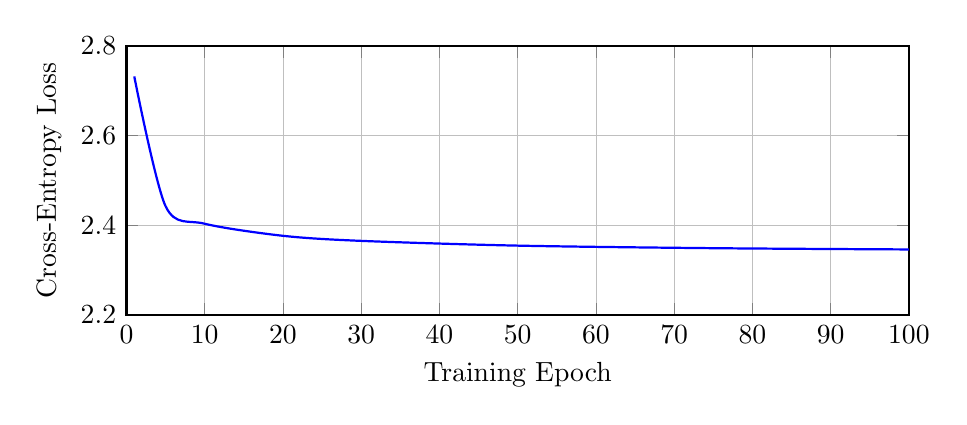
\begin{tikzpicture}
\begin{axis}[
    width=0.95\linewidth,
    height=5cm,
    xlabel={Training Epoch},
    ylabel={Cross-Entropy Loss},
    xmin=0, xmax=100,
    ymin=2.2, ymax=2.8,
    grid=both,
    major grid style={line width=.2pt,draw=gray!50},
    thick
]
\addplot[blue, smooth] coordinates {
    (1,2.7318) (5,2.4426) (10,2.4034) (20,2.3765) (30,2.3652) (50,2.3546) (75,2.3489) (100,2.3461)
};
\end{axis}
\end{tikzpicture}
\caption{LSTM Training Loss (Perplexity) over 100 Epochs. See Appendix C for detailed analysis.}
\label{fig:loss}
\end{figure}

To benchmark the physical efficacy of this pipeline, we simulated a direct attack against Argon2id ($m=65536, t=3, p=4$) utilizing an estimated hash rate of 5,000 Hashes/second, equivalent to a consumer-grade NVIDIA RTX 4090 running optimized recovery tools like Hashcat \cite{hashcat}.

\section{Results and Discussion}

\subsection{Neural Perplexity and Polarization}
Following 100 epochs of training (Time: 43.70 minutes), the model's predictive loss stabilized at $2.34$ (Fig. \ref{fig:loss}). Evaluating the validation lockbox produced a highly polarized distribution of predictability, demonstrating the model's ability to distinguish between cognitive artifacts and genuine randomness.

\begin{table}[htbp]
\caption{Cross-Entropy Loss Rankings (Validation Set). See Appendix C for detailed analysis.}
\begin{center}
\begin{tabular}{@{}llrl@{}}
\toprule
\textbf{Rank} & \textbf{Credential String} & \textbf{Loss} & \textbf{Classification} \\ \midrule
1 & \texttt{qwerty1234567} & 0.5441 & Spatial Walk \\
2 & \texttt{@hotmail.com123} & 0.5646 & Service Template \\
6 & \texttt{iloveforever} & 0.7851 & Semantic/Emotional \\
8 & \texttt{football} & 0.7943 & Dictionary Root \\
\dots & \dots & \dots & \dots \\
99,997 & \texttt{yQg/9\%.I} & 6.7833 & High Entropy \\
99,999 & \texttt{M\%\$R.K.O.} & 7.0367 & High Entropy \\
100,000 & \texttt{l!7h!u\string^\string^} & 7.2075 & High Entropy \\ \bottomrule
\end{tabular}
\label{tab:rankings}
\end{center}
\end{table}

As shown in Table \ref{tab:rankings}, dictionary roots combined with sequential numbers (\texttt{america1234567890}) yielded near-zero perplexity, while strings generated by password managers (\texttt{yQg/9\%.I}) were pushed to the absolute bottom of the attack pipeline.

\subsection{The Hardware Bypass}
By abandoning sequential brute-force methodologies and executing guesses strictly via the LSTM's probabilistically ranked list, the time-to-crack metrics were reduced to critical vulnerabilities.

\begin{itemize}
    \item \textbf{10\% Database Compromise:} Achieved in \textbf{2.00 seconds}.
    \item \textbf{30\% Database Compromise:} Achieved in \textbf{6.00 seconds}.
\end{itemize}

\begin{figure}[htbp]
\centering
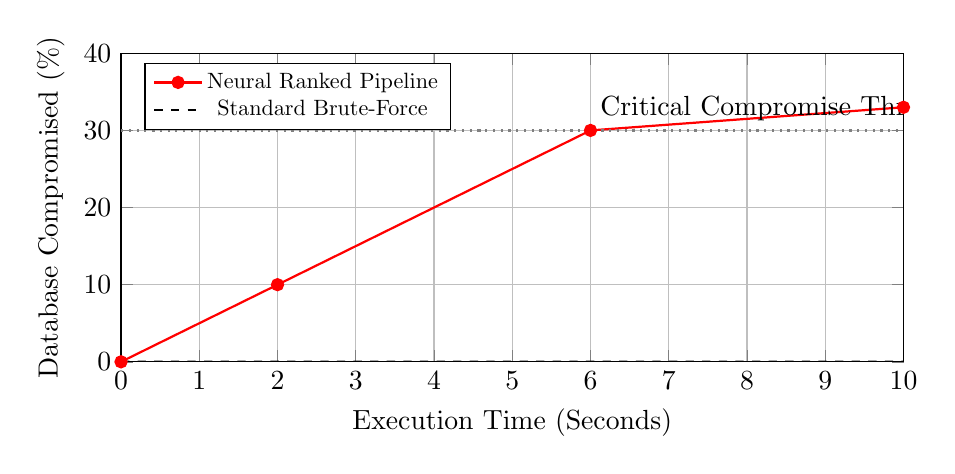
\begin{tikzpicture}
\begin{axis}[
    width=0.95\linewidth,
    height=5.5cm,
    xlabel={Execution Time (Seconds)},
    ylabel={Database Compromised (\%)},
    xmin=0, xmax=10,
    ymin=0, ymax=40,
    grid=major,
    legend pos=north west,
    legend style={nodes={scale=0.8, transform shape}}
]
\addplot[red, thick, mark=*] coordinates {
    (0,0) (2,10) (6,30) (10,33)
};
\addlegendentry{Neural Ranked Pipeline}

\addplot[black, thick, dashed] coordinates {
    (0,0) (10,0.0001)
};
\addlegendentry{Standard Brute-Force}

\addplot[gray, domain=0:10, dotted, thick] {30}; 
\node[above right] at (axis cs:6,30) {Critical Compromise Threshold};
\end{axis}
\end{tikzpicture}
\caption{Comparative rate of network compromise against Argon2id constraints. See Appendix C for detailed analysis.}
\label{fig:compromise}
\end{figure}

These empirical metrics (Fig. \ref{fig:compromise}) demonstrate a catastrophic failure in relying solely on memory-hard hashing. At 5,000 H/s, Argon2id successfully protects the high-entropy passwords at the bottom of the list, but it is mathematically too slow to protect the 30\% of the database that utilized predictable human structures. 

\subsection{The Asymmetry of Modern Exploitation}
The experiment highlights the hardware asymmetry of AI-driven attacks. The intelligence-generation phase---training the 100-epoch model and scoring the validation set---was executed locally on consumer-grade Apple Silicon (MPS) in approximately 43 minutes. Consequently, an attacker does not require continuous access to supercomputing clusters; they only require brief access to GPU hardware to execute the pre-calculated kill list.

\section{Limitations}
While the PCFG-LSTM pipeline is highly lethal against human psychology, it provides zero statistical advantage against mathematical randomness. Passwords generated by cryptographic password managers successfully survived the targeted attack bounds. Furthermore, the model's predictive capabilities are inherently bound to the cultural and linguistic biases present in the specific training corpus (English-centric datasets).

\section{Conclusion}
The security margin of a password cannot be accurately measured by its length or the mathematical boundaries of its character space. Human beings do not select characters uniformly at random. By processing breach corpora through character-level neural networks, attackers can empirically quantify linguistic and structural predictability, drastically collapsing the effective search space.

Our results demonstrate that this neural sorting allows an attacker to completely bypass the hardware limitations of memory-hard KDFs like Argon2id. Compromising 30\% of a target dataset in under six seconds illustrates that current cryptographic cost parameters are drastically undersized when faced with AI-optimized threat actors. To properly defend against these pipelines, security paradigms must shift away from theoretical entropy and begin dynamically evaluating credentials based on neural perplexity at the time of creation.

\begin{thebibliography}{00}
\bibitem{provos1999} N. Provos and D. Mazières, ``A Future-Adaptable Password Scheme,'' \emph{Proceedings of the 1999 USENIX Annual Technical Conference (ATC)}, 1999, pp. 81--92.
\bibitem{argon2} A. Biryukov, D. Dinu, and D. Khovratovich, ``Argon2: new generation of memory-hard functions for password hashing and other applications,'' \emph{IEEE European Symposium on Security and Privacy (EuroS\&P)}, 2016, pp. 292--302.
\bibitem{bonneau2012} J. Bonneau, C. Herley, P. C. van Oorschot, and F. Stajano, ``The quest to replace passwords: A framework for comparative evaluation of web authentication schemes,'' \emph{IEEE Symposium on Security and Privacy}, 2012, pp. 553--567.
\bibitem{weir2009} M. Weir, S. Aggarwal, B. de Medeiros, and B. Glodek, ``Password Cracking Using Probabilistic Context-Free Grammars,'' \emph{IEEE Symposium on Security and Privacy}, 2009, pp. 391--405.
\bibitem{hitaj2019} B. Hitaj, P. Gasti, G. Ateniese, and F. Perez-Cruz, ``PassGAN: A Deep Learning Approach for Password Guessing,'' \emph{Applied Cryptography and Network Security (ACNS)}, 2019, pp. 217--237.
\bibitem{melicher2016} W. Melicher et al., ``Fast, Lean, and Accurate: Modeling Password Guessability Using Neural Networks,'' \emph{25th USENIX Security Symposium}, 2016, pp. 175--191.
\bibitem{rockyou} ``RockYou Data Breach,'' 2009. [Online Dataset].
\bibitem{apple_mps} Apple Inc., ``Metal Performance Shaders Framework,'' Apple Developer Documentation, 2023.
\bibitem{hashcat} J. Steube, ``Hashcat - Advanced Password Recovery,'' 2023. [Online]. Available: https://hashcat.net/hashcat/
\end{thebibliography}

\appendices
\section{Neural Ranking Pipeline (Scoring Engine)}
The following PyTorch script demonstrates the character-level LSTM cross-entropy scoring methodology utilized in Phase 4 of the research to map perplexity and generate the ranked attack pipeline.

\begin{lstlisting}
import torch
import torch.nn as nn

# Hardware optimization for Apple Silicon
device = torch.device("mps" if torch.backends.mps.is_available() else "cpu")

class PasswordLSTM(nn.Module):
    def __init__(self, vocab_size, embed_dim, hidden_dim, num_layers):
        super(PasswordLSTM, self).__init__()
        self.embedding = nn.Embedding(vocab_size, embed_dim, padding_idx=0)
        self.lstm = nn.LSTM(embed_dim, hidden_dim, num_layers, batch_first=True)
        self.fc = nn.Linear(hidden_dim, vocab_size)
        
    def forward(self, x):
        embeds = self.embedding(x)
        lstm_out, _ = self.lstm(embeds)
        return self.fc(lstm_out)

# Initialization & Loss Calculation Function
def evaluate_passwords(val_passwords, model, char2int, vocab_size):
    criterion = nn.CrossEntropyLoss(ignore_index=char2int['<PAD>'], reduction='none')
    password_scores = []
    
    with torch.no_grad():
        for p in val_passwords:
            encoded = [char2int.get(c, char2int['<PAD>']) for c in p]
            inputs = torch.tensor([encoded[:-1]], dtype=torch.long).to(device)
            targets = torch.tensor([encoded[1:]], dtype=torch.long).to(device)
            
            outputs = model(inputs)
            loss_per_char = criterion(outputs.view(-1, vocab_size), targets.view(-1))
            avg_loss = loss_per_char.sum().item() / len(encoded[1:])
            password_scores.append((p, avg_loss))
            
    return sorted(password_scores, key=lambda x: x[1])
\end{lstlisting}

\section{Experimental Hardware Environment}
\begin{itemize}
    \item \textbf{Intelligence Generation Machine:} Apple MacBook Air
    \item \textbf{System on Chip (SoC):} Apple M-Series (Apple Silicon)
    \item \textbf{GPU Acceleration Engine:} Metal Performance Shaders (MPS) via PyTorch \texttt{mps} backend.
    \item \textbf{Target Attack Hardware (Simulated):} NVIDIA RTX 4090 
    \item \textbf{Target KDF:} Argon2id ($m=65536, t=3, p=4$)
    \item \textbf{Estimated Target Hash Rate:} 5,000 H/s
\end{itemize}

\section{Extended Data Analysis}
This section provides expanded analysis for the figures and tables presented in the main text.

\subsection{Analysis of Figure 1 (Training Plateau)}
Figure 1 maps the mathematical reality of machine learning optimization. The model achieved a massive drop in perplexity within the first 20 epochs, effectively mapping the core grammar of the human corpus. The subsequent 80 epochs resulted in a marginal $0.03$ improvement in the cross-entropy loss score. This demonstrates that human structural predictability is relatively shallow and can be mapped computationally with minimal deep-training overhead.

\subsection{Analysis of Table 1 (Polarization)}
Table 1 illustrates the polarization of confidence within the neural network. By Epoch 100, the AI heavily penalized high-entropy strings lacking Markovian transition probabilities (e.g., \texttt{yQg/9\%.I} with a loss of $6.7833$). Conversely, it rewarded sequences mapping cultural frequencies (e.g., dictionary words appended with sequential numbers like \texttt{football} and \texttt{qwerty1234567}) with exceptionally low loss scores.

\subsection{Analysis of Figure 2 (Hardware Bypass)}
Figure 2 contrasts the AI-optimized pipeline against standard sequential brute-forcing. At the Argon2id bottleneck limit of 5,000 H/s, standard brute-forcing remains essentially flat near $0.0001\%$ compromise. The Neural Ranked Pipeline, however, bypasses this hardware defense by feeding the GPU only statistically probable candidates first. Hitting the 30\% critical compromise threshold in 6.00 seconds demonstrates that six seconds is vastly insufficient for automated defensive systems (such as rate-limiting firewalls or account lockouts) to detect and drop an inbound attack before severe lateral compromise occurs.

\end{document}